%!TEX root = ../draft.tex
\begin{figure*}
	\vspace{-20pt}
    \centering
    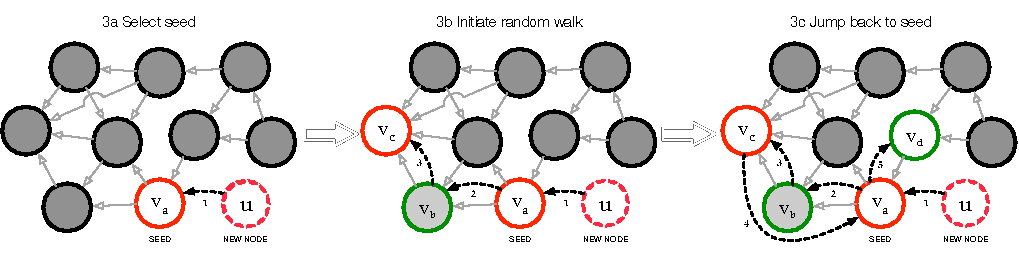
\includegraphics[width=.95\linewidth]{arw}
    \caption{Edge formation in \texttt{ARW}: consider
    an incoming node $u$ with outdegree ${m=3}$ and attribute value {$B(u)=\textsc{red} \in \{\textsc{red},\textsc{green}\}$}.
    In fig. 3a, $u$ joins the network and selects seed $v_a$ via \textsc{Select-Seed}.
    Then, in fig. 3b, $u$ initiates a \textsc{Random-Walk} and traverses from $v_a$ to $v_b$ to $v_c$.
    Finally, $u$ jumps back to its seed $v_a$ and restarts the walk, as shown in fig. 3c.
    Node $u$ halts the random walk after linking to $v_a$, $v_c$ \& $v_d$.
    }
    \label{fig:randomwalk}
	\vspace{-8pt}
\end{figure*}

\section{Attributed Random Walk Model}
\label{sec:Proposed Model}
We propose an Attributed Random Walk (\texttt{ARW}) model to explain the emergence
of key structural properties of real-world networks through {entirely local}
edge formation mechanisms.

Consider a stylized example of how a researcher might go about finding relevant
papers to cite. First, the researcher broadly identifies one or more {relevant}
papers, possibly with the help of external information (e.g. Google
Scholar). These initial set of papers act as seed nodes.  Then, acting under
time and information constraints, she will examine papers cited by the seed and
papers that cite the seed. Thus, she navigates a chain of
backward and forward references to identify {similar}, relevant papers.
Next, through careful analysis, she will cite a subset of these papers. Similarly, users in
online social networks might form new friendships by navigating their social
circle (e.g., friends of friends) to find similar others.

\texttt{ARW} grows a directed network as new nodes join the network. The
mechanism is motivated by the stylized example: an incoming node selects a seed
node and initiates a random walk to explore the network by navigating through
neighborhoods of existing nodes. It halts the random walk after connecting to a
few visited nodes.

In this section, we describe the edge formation mechanisms underlying
\texttt{ARW}, explain how \texttt{ARW} unifies multiple sociological phenomena,
discuss model interpretability and summarize methods required to fit \texttt{ARW}
to network data.
% the observations from empirical data as well as Social Science studies. Then,
% we discuss the methods required to fit \texttt{ARW} to data.


\subsection{Model Description}
\label{sub:Model Description}
The Attributed Random Walk (\texttt{ARW}) model grows a directed network $\{\hat{G}_t\}^T_{t=1}$
in $T$ time steps.
More formally, at every discrete time step $t$, a
new node $u$, with attribute value $B(u)$, joins the network $\hat{G}_t$.
After joining the network, node $u$ forms $m(t)$ edges to
existing nodes.
% At time $t$, $G_t$ consists of ${|V_t|=|V_0|+t}$ nodes,
% ${|E_t|=|E_{t-1}|+m(t)}$ edges and the set of attribute values ${A_t = A_{t-1}
% \cup \{A(u)\}}$.
% The out-degree of incoming nodes increases over time to
% reflect the nonlinear growth and densification of real-world networks.
% We discuss the
% issue of initializing $G_0$, sampling attribute values of inomcing nodes and modeling
% densification in \Cref{sub:Model Fitting}.

The edge formation mechanism consists of two components: \textsc{Select-Seed} and
\textsc{Random-Walk}. As shown in~\Cref{fig:randomwalk}, an incoming node $u$ with attribute value $B(u)$ that joins the
network at time $t$ first selects a seed node using \textsc{Select-Seed}:
\\\\
\tikzstyle{background rectangle}=[thin,draw=black]
\begin{tikzpicture}[show background rectangle]
	\node[align=left, text width=.93\linewidth, inner sep=.5em]{
		(1) With probability $\nicefrac{\psame}{\psame+\pdiff}$, randomly select a seed node
		from existing nodes that have the same attribute value, $B(u)$.

		\vspace{1mm}
		(2) Otherwise, with probability $\nicefrac{\pdiff}{\psame+\pdiff}$, randomly select a seed node from existing nodes that
		do \textit{not} have the same attribute value, $B(u)$.
	};
	\node[xshift=3ex, yshift=-.7ex, overlay, fill=white, draw=white, above
	right] at (current bounding box.north west) {
		\textsc{Select-Seed}
	};
\end{tikzpicture}

% The attribute parameter $p_a$ incorporates the attribute preferences of incoming nodes
% into the model.

\textsc{Select-Seed} accounts for homophilic preferences of incoming nodes using
parameters $\psame$ and $\pdiff$, which incorporates attribute preferences of incoming nodes.
As shown in~\Cref{fig:randomwalk}, after selecting
the seed node, $u$ initiates a
random walk using \textsc{Random-Walk} to form $m(t)$ links.
The \textsc{Random-Walk} mechanism consists of four parameters: attribute-based parameters
$\psame$ \& $\pdiff$ model edge formation decisions and the jump parameter $\pjump$ \&
out-link parameter $\pout$ characterize random walk traversals:
\\\\
\tikzstyle{background rectangle}=[thin,draw=black]
\begin{tikzpicture}[show background rectangle]
	\node[align=left, text width=.93\linewidth, inner sep=.5em]{
		(1) At each step of the walk, new node $u$ visits node $v_i$.
		\begin{itemize}
			\item If $B(u)=B(v_i)$, $u$ links to $v_i$ with probability $\psame$
			\item Otherwise, $u$ links to $v_i$ with probability $\pdiff$
		\end{itemize}

		\vspace{1mm}
		(2) Then, with probability $\pjump$, $u$ jumps back to seed $s_u$.

		\vspace{1mm}
		(3) Otherwise, with probability ${1-\pjump}$, $u$ continues to walk.
		It picks an outgoing edge with prob. $\pout$ \textit{or}
		an incoming edge with prob. $1-\pout$ to visit a neighbor of $v_i$.

		\vspace{1mm}
		(4) Steps 1-3 are repeated until $u$ links to $m(t)$ nodes.
	};
	\node[xshift=3ex, yshift=-.7ex, overlay, fill=white, draw=white, above
	right] at (current bounding box.north west) {
		\textsc{Random-Walk}
	};
\end{tikzpicture}

When attribute data is absent, \texttt{ARW} simplifies further, as
a single link parameter $\plink$ replaces both attribute parameters $\psame$ \& $\pdiff$.
\textsc{Select-Seed} reduces to uniform seed selection and in
\textsc{Random-Walk}, the probability of linking to visited nodes equals $\plink$.
%  \textsc{Select-Seed} simplifies to selecting an existing
% node uniformly at random and \textsc{Random-walk} simplifies to selecting an existing
% node uniformly at random.\texttt{ARW} only requires a single link
% parameter $\plink$, instead of both $\psame$ \& $\pdiff$. Additionally,


Note that \texttt{ARW} has two exogenous parameters: the out-degree
$m(t)$ and attribute $B(u)$ of incoming nodes.
The attribute distribution varies with time as new attribute values (e.g., journals) crop up, necessitating an exogenous
parameter. The parameter $m(t)$ is the mean-field value
of out-degree $m$ at time $t$ in the observed network.
While it is straightforward to model $m(t)$
endogenously by incorporating a densification power-law \texttt{DPL} exponent,
exogenous factors (e.g., venue, topic) may influence node out-degree.
%  similar to the parameter $m$ in the classic Preferential-Attachment
% model~\cite{barabasi1999emergence}, except that $m(t)$ is the mean-field value
% of out-degree $m$ at time $t$ in the observed network.
% While it is straightforward to model $m(t)$
% endogenously by incorporating a densification power-law \texttt{DPL} exponent
% to \texttt{ARW}, we decided against it, since exogenous factors may
% also explain changes to $m(t)$. For example, conference venue and paper topic can
% influence the number of citations in a paper. Moreover, our analysis indicates
% that papers that join networks earlier tend to have fewer citations on average,
% perhaps explained by availability of {fewer} papers to cite.

Next, we explain how each parameter is necessary to conform to normative
behavior of individuals in evolving networks.

\subsection{\texttt{ARW} and Normative Behavior}
\label{sub:Model Interpretation}
The Attributed Random Walk model unifies multiple sociological phenomena
into its edge formation mechanisms.

\newtheoremstyle{exampstyle}
  {2pt} % Space above
  {2pt} % Space below
  {\itshape} % Body font
  {} % Indent amount
  {\bfseries} % Theorem head font
  {.} % Punctuation after theorem head
  {.25em} % Space after theorem head
  {} % Theorem head spec (can be left empty, meaning `normal')

\theoremstyle{exampstyle} \newtheorem{ph}{Phenomenon}

\begin{ph}
	(Limited Resources) Individuals are boundedly rational~\cite{simon1972theories,gigerenzer1996reasoning,lipman1995information}
	actors that form edges under constraints of limited information, partial network access and finite cognitive capacity.
\end{ph}
\texttt{ARW} uses random walk traversals to incorporate constraints of limited information
and partial network access. A new node $u$ selects a seed node from which it
initiates a biased random walk. Then, $u$ uses simple rules to connect to each visited
nodes probabilistically and halts the walk after forming $m(t)$ edges, as shown in~\Cref{fig:randomwalk}. Random walks require information only about the
1-hop neighborhood of visited nodes, thereby accounting for  the constraints of limited information and partial network access.

\begin{ph}
	(Structural Constraints) Structural factors such as network distance
	act as constraints that limit edge formation to proximate nodes.  \cite{35626}
\end{ph}

We incorporate structural constraints into \texttt{ARW} using $\pjump$, the probability with
which a new node jumps back to its seed node after each step of the random walk. This implies
that the probability with which the new node is at most $k$ steps from its seed node is $(1-\pjump)^k$;
as a result, $\pjump$ controls the extent to which nodes' random walks explore the network to form edges.

\begin{ph}
	(Triadic Closure) Nodes with common neighbors have an
	increased likelihood of forming a connection. \cite{simmel1950sociology}
\end{ph}

When attribute data is absent, \texttt{ARW} controls
the effect of triadic closure on link formation using $\plink$ since
a new node $u$ closes a triad through its random walk by linking to both, a visited node
and its neighbor, with probability proportional to $\plink^2$.
Similarly, in attributed networks, the probability of triad completion equals $pq$,
where $p$ and $q$ can equal $\psame$ or $\pdiff$, depending on the attribute values of
$u$ and the visited nodes.

\begin{ph}
	(Attribute Homophily) Nodes that have similar attributes are more likely
	to form a connection. \cite{mcpherson2001birds}
\end{ph}
The attribute parameters $\psame$ and $\pdiff$ modulate
attribute assortativity. When $\psame > \pdiff$, nodes are more likely to connect if they share
the same attribute value, thereby resulting in a homophilic network over time. Similarly,
$\psame < \pdiff$ and $\psame=\pdiff$ make edge formation heterophilic and attribute agnostic respectively.

\begin{ph}
	(Preferential Attachment) Nodes tend to link to high degree nodes that have more
	visibility. \cite{barabasi1999emergence}
\end{ph}
\texttt{ARW} controls preferential attachment by adding structural bias to the
random walk traversal using outlink parameter $\pout$, instead of relying on the
global degree distribution. Random walks that traverse outgoing edges only
(i.e., $\pout =1$) eventually visit old nodes that tend to have high in-degree.
Similarly, random walks that traverse incoming edges only (i.e., $\pout=0$) visit
recently joined nodes that tend to have low indegree. As a result, we use
$\pout$ to adjust the effect of preferential attachment on edge formation.

To summarize: \texttt{ARW} incorporates five well-known sociological
phenomena--- bounded rationality; structural constraints; triadic closure;
attribute homophily; preferential attachment---into a single edge formation
mechanism based on random walks.

% Random walks inherently account for
% limited information and partial network access. Furthermore, the jump parameter $p_j$, attribute parameter $p_a$,
% rate parameter $\alpha$ and out parameter $p_o$ incorporate the effect of structural constraints,
% homophily, triadic closure and preferential attachment respectively.

\subsection{Model Interpretability}
In addition to unifying multiple sociological phenomena, \texttt{ARW} parameters
intuitively modulate global structural properties:
in-degree distribution, local clustering, path length and attribute assortativity.

In order to understand how global network properties vary as functions of
\texttt{ARW} parameters, we explore the parameter space of the model. As
described in~\Cref{sub:Model Description}, \texttt{ARW} uses two
parameterizations to model networks with or without attribute data. We analyze
network structure and attribute assortativity using $(\plink, \pjump, \pout)$
and $(\psame, \pdiff, \pjump, \pout)$ respectively.

\begin{figure}[t]
 % \vspace{-10pt}
 \centering
 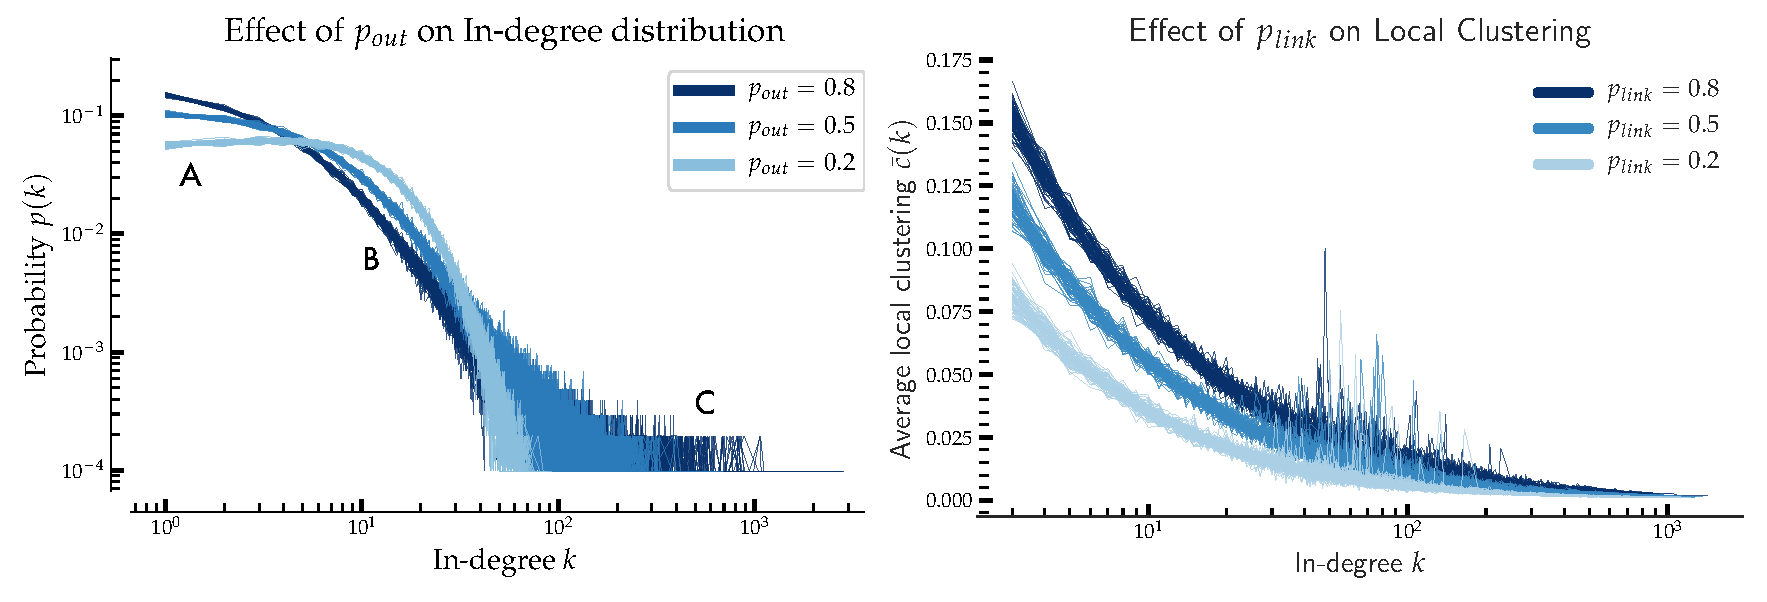
\includegraphics[width=\columnwidth]{inter1}
 \caption{
 	Increasing $\pout$ and $\plink$
	raises incoming nodes' biases towards high-degree and proximate nodes
	and subsequently leads to in-degree distributions with heavier tails
	and neighborhoods with higher clustering.
 }
 \label{fig:inter1}
 \vspace{-10pt}
\end{figure}

\Cref{fig:inter1} illustrates how in-degree distribution and local clustering depend on $\pout$ and $\plink$ respectively.
Increasing $\pout$ steers random walks towards older nodes that tend to have higher in-degree
Over time, as more nodes join the network, initial differences in degree amplify, resulting in heavy-tailed distributions.
Consequently, as shown in ~\Cref{fig:inter1}, increasing $\pout$ from $0.2$ to $0.8$ shifts the probability
mass from average degree nodes (\texttt{B}) to hubs (\texttt{C}) and nodes with low indegree (\texttt{A}).
Similarly, local clustering increases as a function of $\plink$, which implicitly
controls the rate at which new nodes close triads via random walks by linking to adjacent nodes.

\begin{figure}[H]
 % \vspace{-10pt}
 \centering
 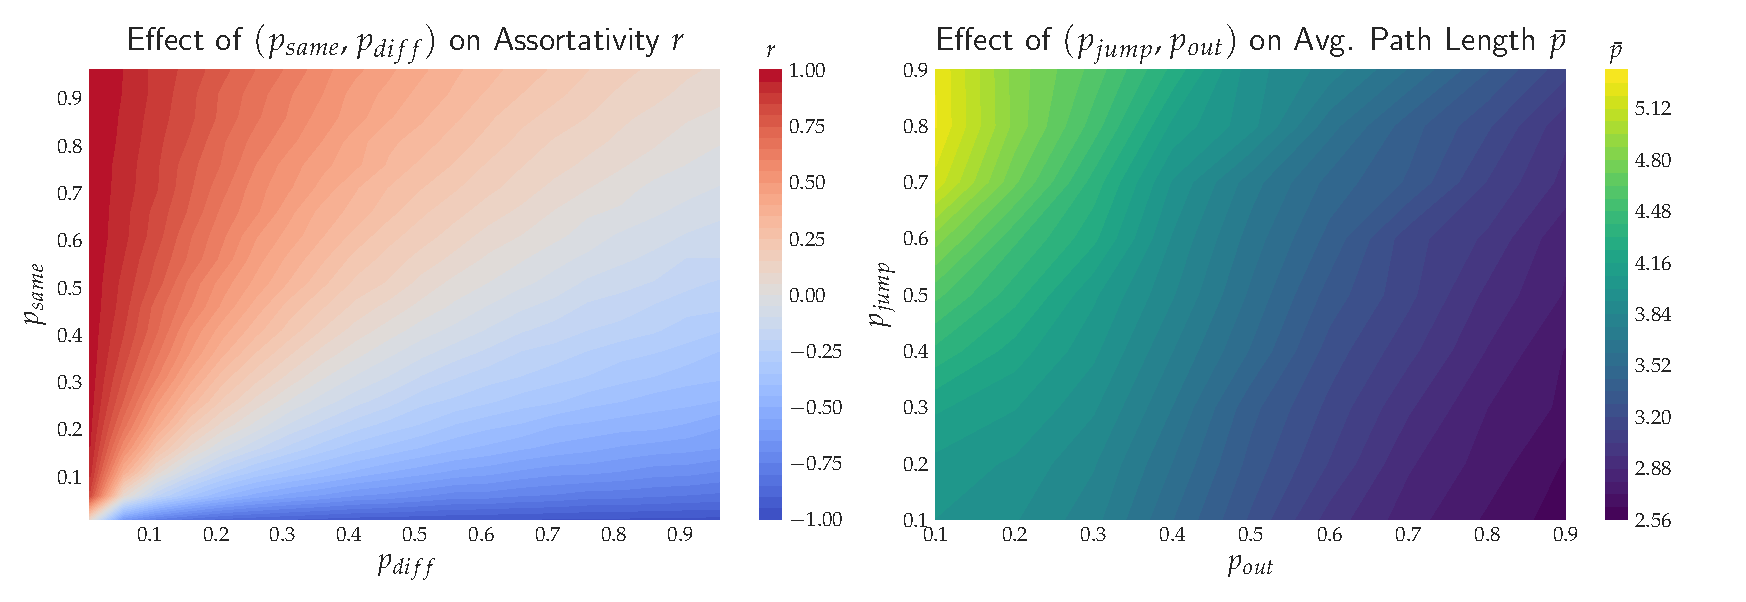
\includegraphics[width=\columnwidth]{inter2}
 \caption{
 	Increasing $\psame-\pdiff$ makes edge formation more homophilic
	and leads to higher assortativity. Decreasing $\pjump$ while increasing
	$\pout$ leads to longer random walks towards older, higher degree nodes,
	and subsequently shortens average path length.
 }
 \label{fig:inter2}
 % \vspace{-10pt}
\end{figure}

\harshay{TODO: explain \Cref{fig:inter2} and conclude (2 paras)}


\subsection{Model Fitting}
\label{sub:Model Fitting}

We now briefly describe methods to estimate model parameters,
initialize $\hat{G}$, densify $\hat{G}$ over time and sample nodes' attribute values.

\textit{Parameter Estimation}.
The parameter estimation task consists of finding the set of parameters values
for $(\psame, \pdiff, \pjump, \pout)$ that best preserve the structural properties of an
observed network $G$. We use a straightforward grid search method to estimate
the four parameters using evaluation metrics and selection criterion described in~\Cref{sub:Experimental Setup}.
Note that other derivative-free optimization methods such as the Nelder-Mead~\cite{nelder1965simplex} method
can be used to speed-up parameter estimation.

\textit{Initialization}. The edge formation mechanism in \texttt{ARW} is
sensitive to a large number of weakly connected components (\texttt{WCC}s) in the
initial network $\hat{G}_0$ because incoming nodes can only form edges to nodes
in the same \texttt{WCC}. To ensure that $\hat{G}_0$ is weakly
connected, we perform an undirected breadth-first search on the observed,
to-be-fitted network $G$ that starts from the oldest node and terminates after
visiting $0.1\%$ of the nodes. The initial network $\hat{G}_0$ is the small \texttt{WCC}
induced from the set of visited nodes.
% Simpler initialization methods
% such as sampling $\hat{G}_0$ from the Erdos-Renyi model or Watts-Strogatz model
% yield similar results.


\textit{Node Out-degree}.
The out-degree of incoming nodes increases  nonlinearly over time in real-world networks.
We coarsely reflect the rate of growth in the observed network $G$ as follows.
Each incoming node $u$ that joins $\hat{G}$ at time $t$ corresponds to some
node that joins the observed network $G$ in year $y(t)$; the number of edges $m(t)$
that $u$ forms is equal to the average out-degree of nodes that join $G$ in year $y(t)$.

\textit{Sampling Attribute Values}.
The distribution over nodal attribute values $P_{\textsc{g}}(B)$ tends to change over time.
% For instance, the attribute distribution over journals in the \texttt{APS} citation
% network changes over time as old journals decay in popularity and new journals gain traction.
The change in the attribute distribution over time is an exogenous factor and varies for every network.
Therefore, we sample the attribute value $B(u)$ of node $u$, that joins $\hat{G}$ at time
$t$, from $P_{\textsc{g}}(B{\mbox{ | year}=y(t)})$, the observed attribute
distribution conditioned on the year of arrival of node $u$.

To summarize, \texttt{ARW}
intuitively describes how individuals form edges under resource constraints.
\texttt{ARW} uses four parameters ---$\psame$, $\pdiff$, $\pjump$, $\pout$--- to incorporate
individuals' biases towards similar, proximate and high degree nodes.
% We note that a mathematical analysis of \texttt{ARW} appears to lead to novel
% theoretical questions about random walks on directed graphs.
% Unfortunately, unlike the case of undirected graphs, there is no
% analytical closed form expression for stationary distributions of random walks
% on general directed graphs, thereby making the analysis of random walk models
% like \texttt{ARW} quite complex. \harshay{Improve theory justification
Next, we discuss our experiments on the performance of $\texttt{ARW}$
in accurately preserving {multiple} structural and attribute properties of real networks.

